
\chapter{結果}\label{chap_result}
%loss,accのグラフは全て.
%前処理を行った場合は,その画像の一例も載せる
%モデルの画像(appendixの方がいいかもしれないです)
%各sectionで異なる場合は各sectionで載せましょう
%なるべくpdfで保存しましょう

\section{古典的な画像処理手法による識別精度評価}
%楕円検出の塗った画像
%円検出の画像
\begin{figure}[H]
	\centering
	\includegraphics[width=\linewidth]{fig/circle_detection}
	\caption{Detection of circle.}
	\label{fig:circle_detection}
\end{figure}

\begin{figure}[H]
	\centering
	\includegraphics[width=\linewidth]{fig/eclips_detection}
	\caption{Detection of ellipse}
	\label{fig:ellipse_detection}
\end{figure}

\fig{circle_detection}が円検出を利用して正常の構造を検出した結果である.緑色の円の部分が円検出された領域を示している.真円にフィッティングしているため綺麗な円構造のみの検出となり,正常でも検出できていない部分が多くなっている.全体的に正常領域で円検出が多く行われ,腫瘍領域では円検出結果が少なくなる結果となったが,腫瘍部分も円検出されている部分が一部ある.

\fig{ellipse_detection}は楕円検出を行った結果である.円検出よりも正常領域の検出が増えたことが分かる.楕円検出がされた領域の多いところほど正常の領域で,楕円検出が少ない領域が腫瘍であるという傾向を捉えることができた.古典的な画像処理の利点は,画像検出の理由が明確に説明できることである.このような円検出や楕円検出であれば,円形度を算出することができるので,深層学習を用いた結果よりも透明性がある.しかしながら,明確な輪郭で無ければ検出できない場合が多く検出精度に限界があることから,これでは腫瘍の見落とし防止に利用することができない.そこで古典的な画像処理の性能を上回る,深層学習を利用するが必要であると分かる.


\section{教師あり学習による識別精度評価}
教師あり学習では,まず2次元画像で,元画像のまま学習した場合と,擬似HE変換した画像を学習する場合,さらに事前学習を行った場合で比較を行った.

\begin{figure}[H]
	\centering
	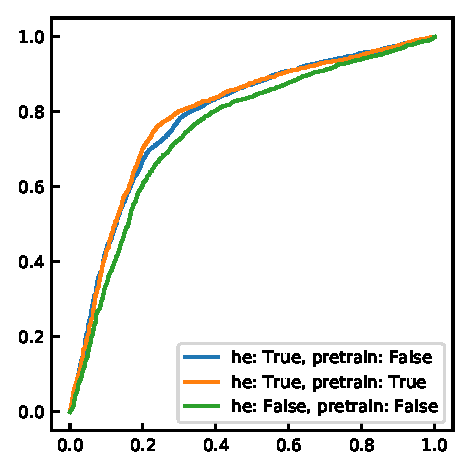
\includegraphics[width=0.5\linewidth]{fig/chapter4/2dcnn_preprocessing}
	\caption{ROC for 2DCNN with different preprocessing}
	\label{fig:2dcnnpreprocessing}
\end{figure}

\begin{figure}[H]
	\centering
	\begin{minipage}[b]{0.45\columnwidth}
	\centering
	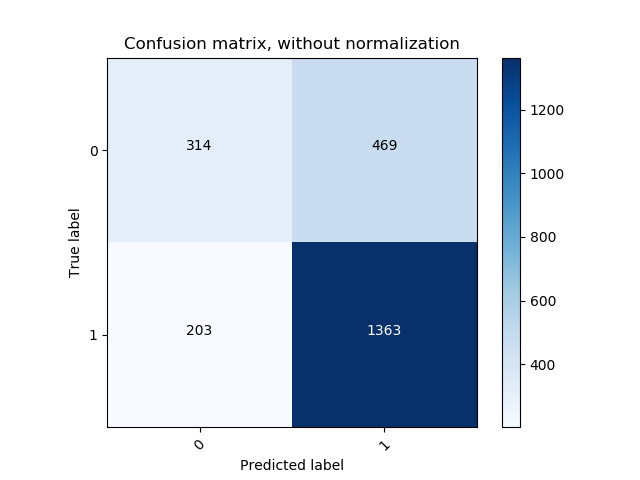
\includegraphics[clip, width=\linewidth]{fig/chapter4/count_pretrain_False_he_False}
	\subcaption{pretrain: Flase, he transform: False}
	\label{fig:count_no_preprocess}
    \end{minipage}
	\begin{minipage}[b]{0.45\columnwidth}
		\centering
		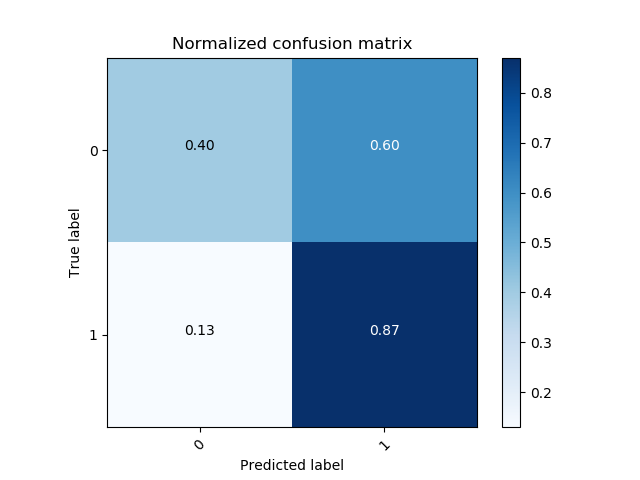
\includegraphics[clip, width=\linewidth]{fig/chapter4/pretrain_False_he_False}
		\subcaption{pretrain: Flase, he transform: False}
		\label{fig:no_preprocess}
	\end{minipage}
	\begin{minipage}[b]{0.45\columnwidth}
	\centering
	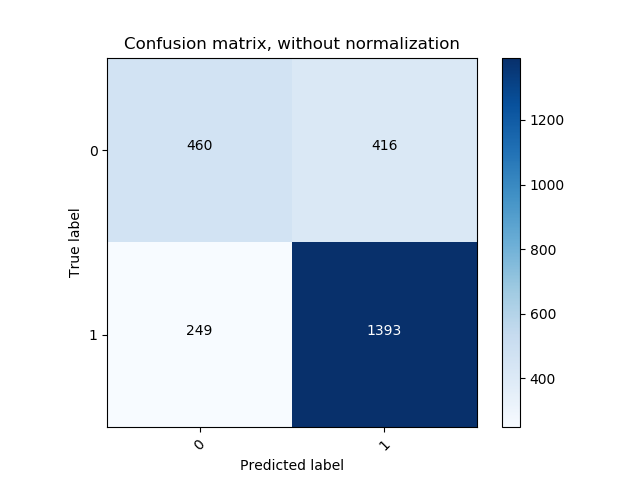
\includegraphics[clip, width=\linewidth]{fig/chapter4/count_pretrain_False_he_True}
	\subcaption{pretrain: Flase, he transform: True}
	\label{fig:count_he_preprocess}
    \end{minipage}
	\begin{minipage}[b]{0.45\columnwidth}
		\centering
		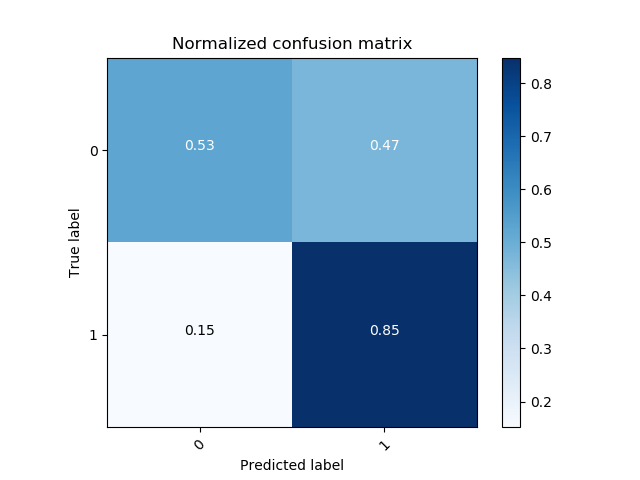
\includegraphics[clip, width=\linewidth]{fig/chapter4/pretrain_False_he_True}
		\subcaption{pretrain: Flase, he transform: True}
		\label{fig:he_preprocess}
	\end{minipage}
	\begin{minipage}[b]{0.45\columnwidth}
	\centering
	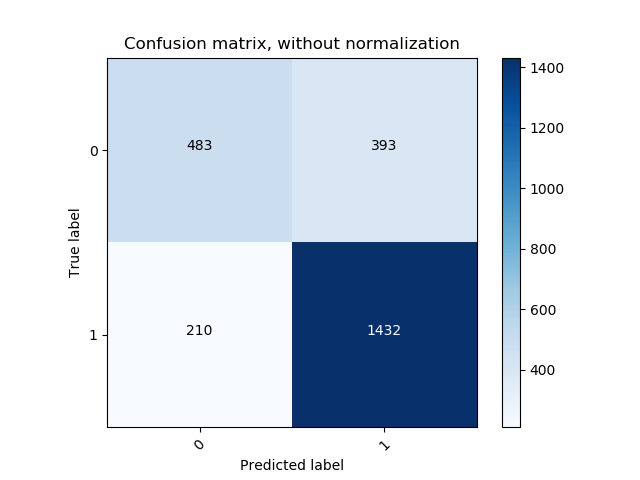
\includegraphics[clip, width=\linewidth]{fig/chapter4/count_pretrain_True_he_True}
	\subcaption{pretrain: True, he transform: True}
	\label{fig:count_pretrain_preprocess}
    \end{minipage}
	\begin{minipage}[b]{0.45\columnwidth}
		\centering
		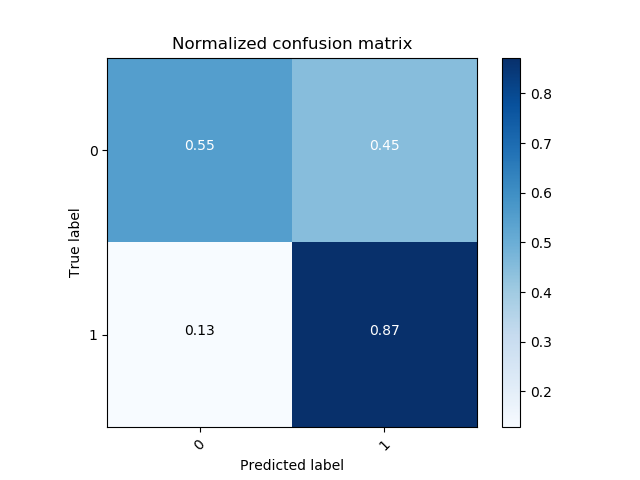
\includegraphics[clip, width=\linewidth]{fig/chapter4/pretrain_True_he_True}
		\subcaption{pretrain: True, he transform: True}
		\label{fig:pretrain_preprocess}
	\end{minipage}
	
	\caption{Confusion Matrix for 2DCNN with different preprocessing}
	\label{fig:2d_preprocess_matrix}
	
\end{figure}

前処理を何も行わない場合が\fig{2dcnnpreprocessing}の緑のプロットでありROCの評価指数である.AUCはhogeで一番認識精度が低かった.また\fig{no_preprocess}のように腫瘍は87\%の精度で検出できているが,正常は40\%の精度でしか検出できていなかった.

ここで腫瘍の見落としとなる偽陰性の割合が13\%と低く,偽陽性が高くなっていることが分かる.このようになった理由は,深層学習の学習方法に理由がある.今回学習に用いたデータで正常は,783枚であるのに対して,腫瘍の学習データの枚数は1566枚である.正常の画像よりも腫瘍の画像を2倍多く学習に利用することで,腫瘍の検出がより重要視されるモデルになったのである.これは,病変の見落としリスクを防止するためには,非常に良い結果となった.

腫瘍の見落とし率が低いことは良いが,正常を腫瘍と判断する割合が高すぎるのでこれを正しく正常画像を正常と判断できるようにしなくてはならない.

ここで前処理として擬似HE変換を行って学習した結果(\fig{he_preprocess})と,擬似HE変換した後に,事前学習も行った時の学習結果(\fig{pretrain_preprocess})から,前処理をすることで腫瘍の見落としリスクを低くしたまま,正常画像を正しく認識することができるようになった.

\subsection*{モデルの比較}
InceptionV3とXception, InceptionResnetV2を比較して,どのネットワークが認識精度が高いのかを実験した.

\begin{figure}[H]
	\centering
	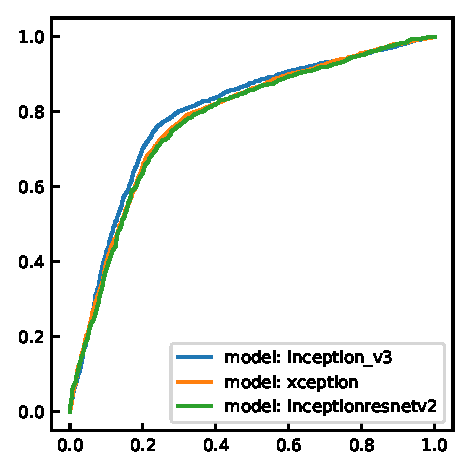
\includegraphics[width=0.7\linewidth]{fig/chapter4/2dcnn_model}
	\caption{Comparing deep learning models}
	\label{fig:2dcnnmodel}
\end{figure}

先行研究でも利用されているように,今回の研究に用いた検体データでもInceptionV3がもっともAUCが大きくなるディープラーニングのモデルであることが分かった.XceptionやInceptionResnNetV2など様々なディープラーニングのモデルが研究され利用されているが,一般物体認識では,InceptionResNet,Xception, InceptionV3の順番に精度が高いことが報告されているが,実際のデータが変化するごとに,どのモデルがもっとも精度が高くなるかを事前に判断することが難しいことが分かった.

\subsection{3次元画像解析}
3DCNNは,学習する際の訓練パラメータが多すぎて,学習が収束しない点や,メモリが大きくてGPUに乗らないという問題があり,時系列解析で行われているLSTMやGRUまた,BidirectionalなGRUをモデルの比較として利用した.

\begin{figure}[H]
	\centering
	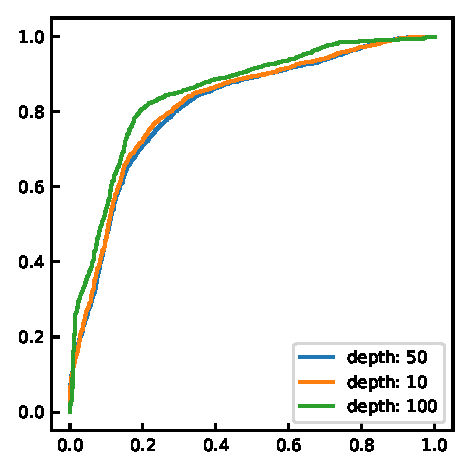
\includegraphics[width=0.7\linewidth]{fig/chapter4/3d/roc/depth_all.pdf}
	\caption{depth}
	\label{fig:depthall}
\end{figure}

\begin{figure}[H]
	\centering
	
	\begin{minipage}[b]{0.45\columnwidth}
		\centering
		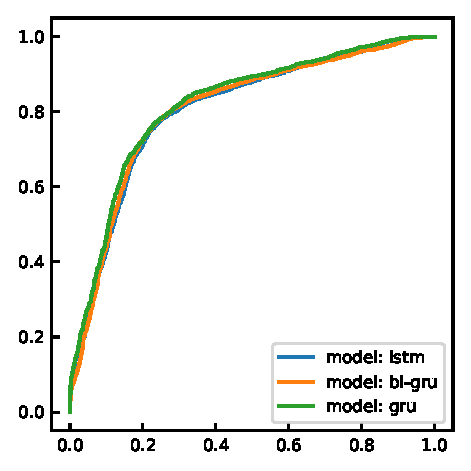
\includegraphics[clip, width=\linewidth]{fig/chapter4/3d/roc/depth_10.pdf}
		\subcaption{depth: 10}
		\label{fig:}
	\end{minipage}
	\begin{minipage}[b]{0.45\columnwidth}
		\centering
		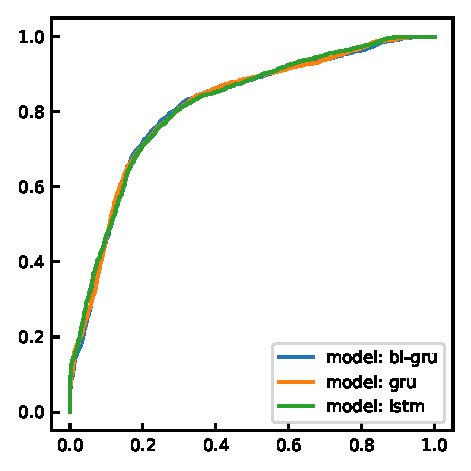
\includegraphics[clip, width=\linewidth]{fig/chapter4/3d/roc/depth_50.pdf}
		\subcaption{depth: 50}
		\label{fig:}
	\end{minipage}
	\begin{minipage}[b]{0.45\columnwidth}
		\centering
		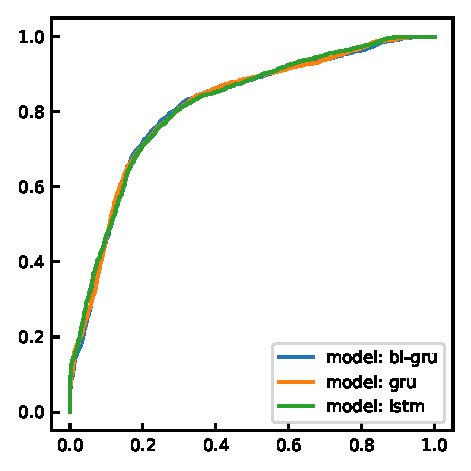
\includegraphics[clip, width=\linewidth]{fig/chapter4/3d/roc/depth_100.pdf}
		\subcaption{depth: 100}
		\label{fig:}
	\end{minipage}
	
	\caption{ROC curve with different depth}
	\label{fig:2dcnn+LSTM_roc}
	
\end{figure}

ここでLSTMやGRU, Bi-GRUといったモデルによる精度の差は,ほとんどなかった.GRUがもっとも訓練パラメータが少ないので学習時間や推論時間を早くすることができる.そのため今後はGRUを使って学習をすると効率が良いことが分かった.

深さ方向に10, 50, 100と増やしていくと腫瘍と正常の認識精度を向上させることができた.これは,正常の場合だと腺菅構造が深さ方向に一定に変化するのに対して,腫瘍の場合は構造が乱れているので変化も不規則であるという性質など,3次元的な構造を捉えながら学習することができたため,認識精度が上がったと言える.

\begin{figure}[H]
	\centering
	\begin{minipage}[b]{0.45\columnwidth}
		\centering
		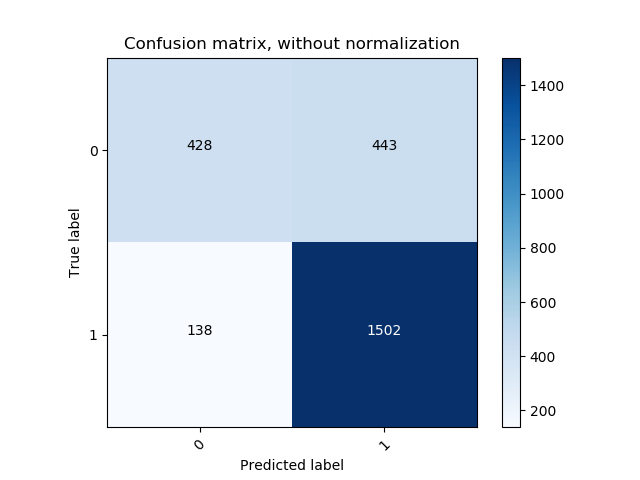
\includegraphics[clip, width=\linewidth]{fig/chapter4/3d/confusion_matrix/count_confusion_matrix_False_10_gru}
		\subcaption{confusion matrix depth 10}
		\label{fig:count_10}
	\end{minipage}
	\begin{minipage}[b]{0.45\columnwidth}
		\centering
		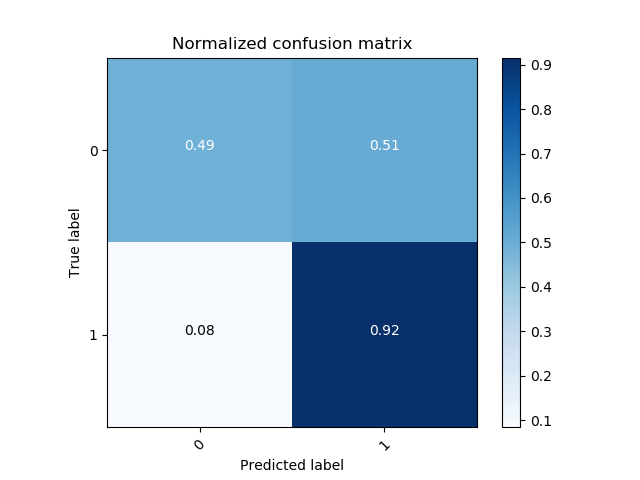
\includegraphics[clip, width=\linewidth]{fig/chapter4/3d/confusion_matrix/normalized_confusion_matrix_False_10_gru}
		\subcaption{normalized matrix depth 10}
		\label{fig: depth10}
	\end{minipage}
	\begin{minipage}[b]{0.45\columnwidth}
		\centering
		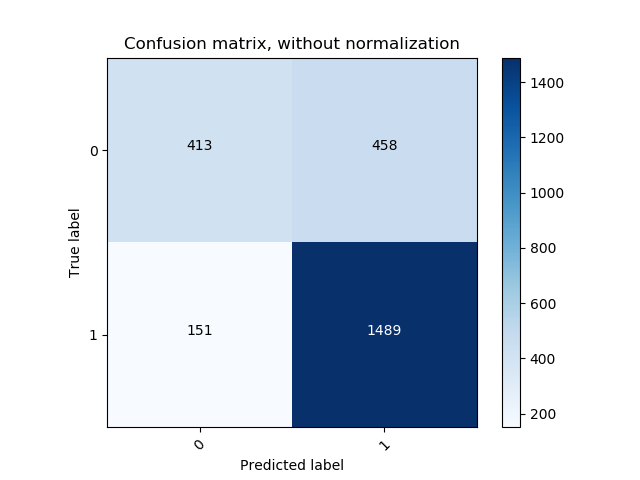
\includegraphics[clip, width=\linewidth]{fig/chapter4/3d/confusion_matrix/count_confusion_matrix_False_50_gru}
		\subcaption{confusion matrix depth 50}
		\label{fig: count_he_preprocess}
	\end{minipage}
	\begin{minipage}[b]{0.45\columnwidth}
		\centering
		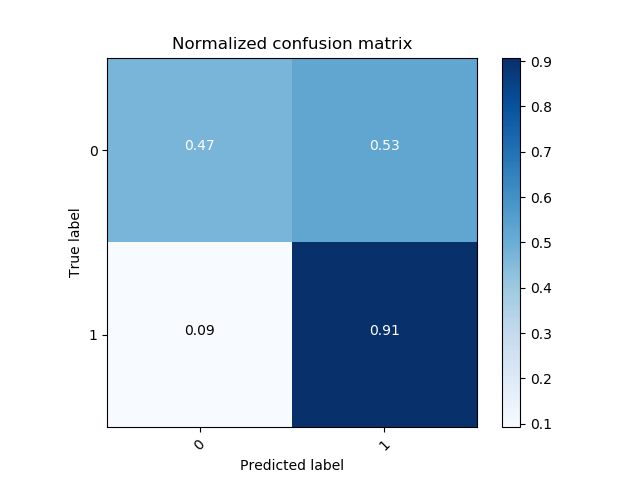
\includegraphics[clip, width=\linewidth]{fig/chapter4/3d/confusion_matrix/normalized_confusion_matrix_False_50_gru}
		\subcaption{normalized matrix depth 50}
		\label{fig: he_preprocess}
	\end{minipage}
	\begin{minipage}[b]{0.45\columnwidth}
		\centering
		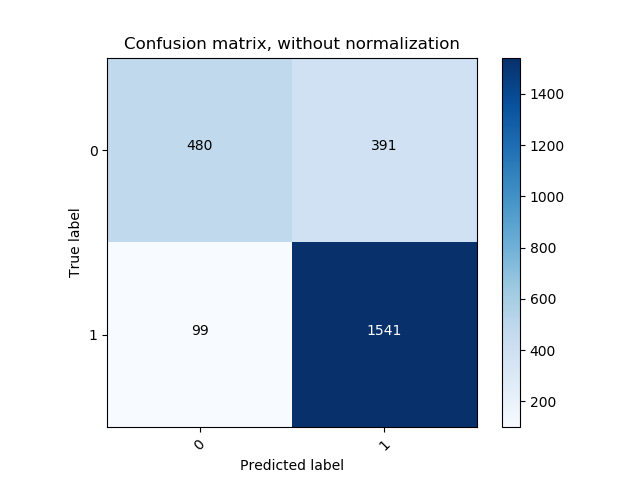
\includegraphics[clip, width=\linewidth]{fig/chapter4/3d/confusion_matrix/count_confusion_matrix_False_100_gru}
		\subcaption{confusion matrix depth 100}
		\label{fig: count_pretrain_preprocess}
	\end{minipage}
	\begin{minipage}[b]{0.45\columnwidth}
		\centering
		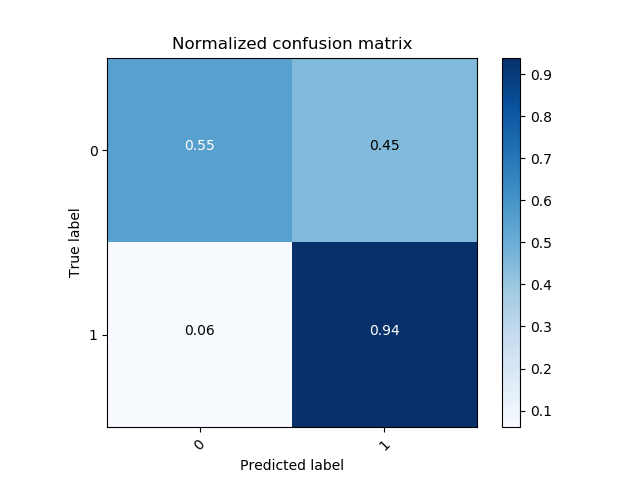
\includegraphics[clip, width=\linewidth]{fig/chapter4/3d/confusion_matrix/normalized_confusion_matrix_False_100_gru}
		\subcaption{normalized matrix depth 100}
		\label{fig: pretrain_preprocess}
	\end{minipage}
	
	
	\caption{Confusion Matrix for 2DCNN with different preprocessing}
	\label{fig:gru_matrix}
	
\end{figure}

\section{教師なし学習による識別精度評価}
\subsection{AutoEncoder}

\begin{figure}[H]
	\centering
	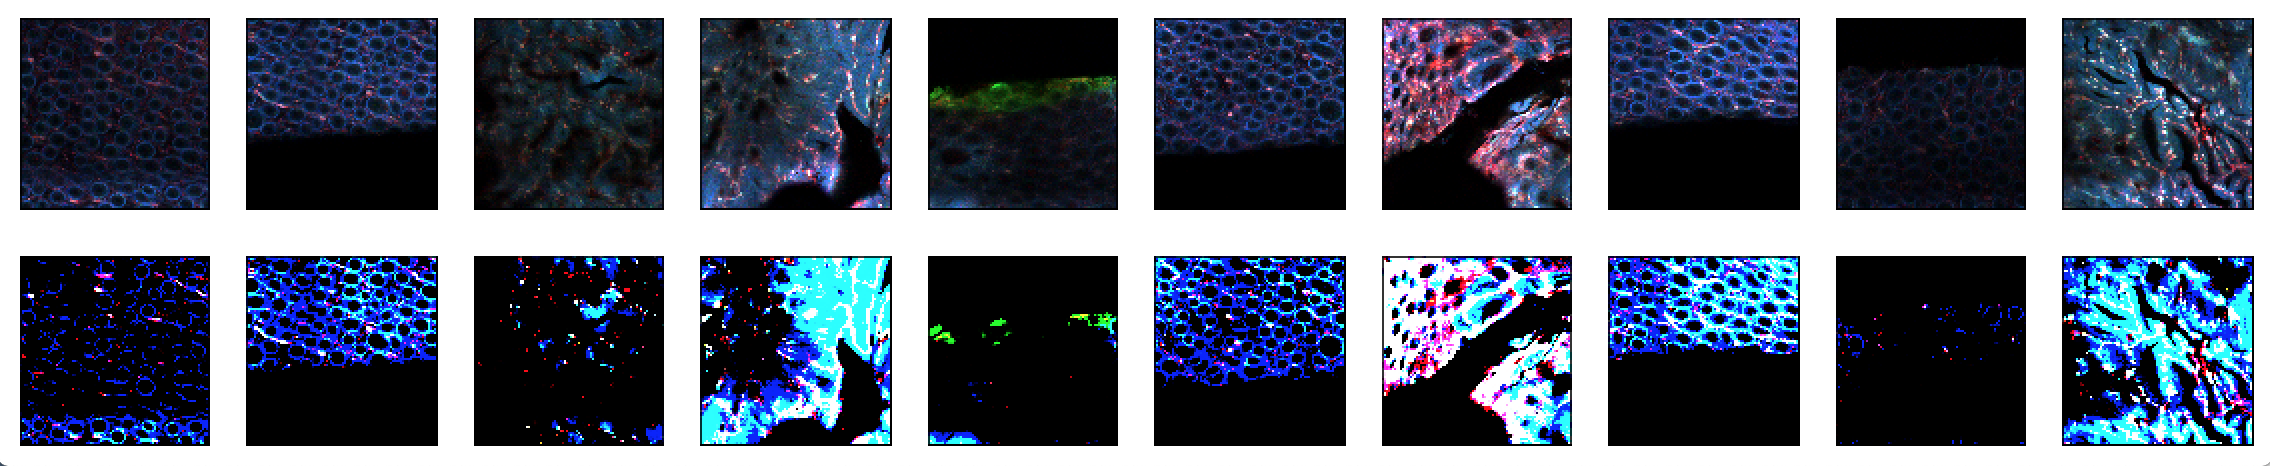
\includegraphics[width=0.9\linewidth]{fig/chapter4/unet_ae}
	\caption{Auto Encoder}
	\label{fig:unetae}
\end{figure}


\subsection{GAN}

\begin{figure}[H]
	\centering
	
	\begin{minipage}{0.24\columnwidth}
		\centering
		
\includegraphics[clip, width=\linewidth]{fig/generative_adversarial_nets/0000_0000}
		\subcaption{epochs = 0}
		\label{fig:}
	\end{minipage}
	\begin{minipage}{0.24\columnwidth}
		\centering
		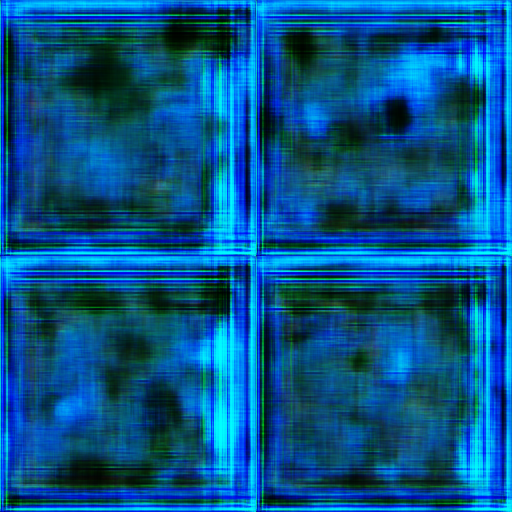
\includegraphics[clip, width=\linewidth]{fig/generative_adversarial_nets/0079_0000}
		\subcaption{epochs = 79}
		\label{fig:}
	\end{minipage}
	\begin{minipage}{0.24\columnwidth}
		\centering
		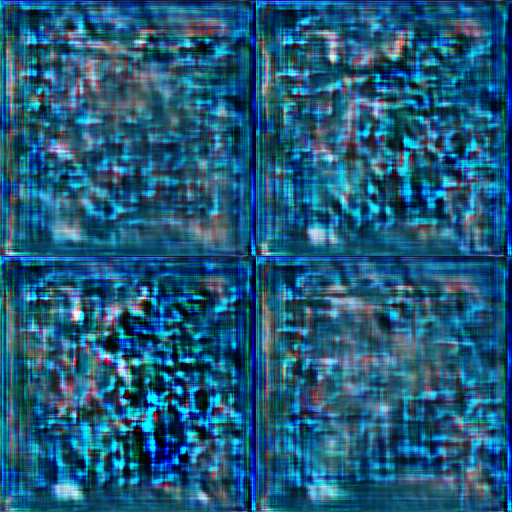
\includegraphics[clip, width=\linewidth]{fig/generative_adversarial_nets/0641_0000}
		\subcaption{epochs = 641}
		\label{fig:}
	\end{minipage}
	\begin{minipage}{0.24\columnwidth}
		\centering
		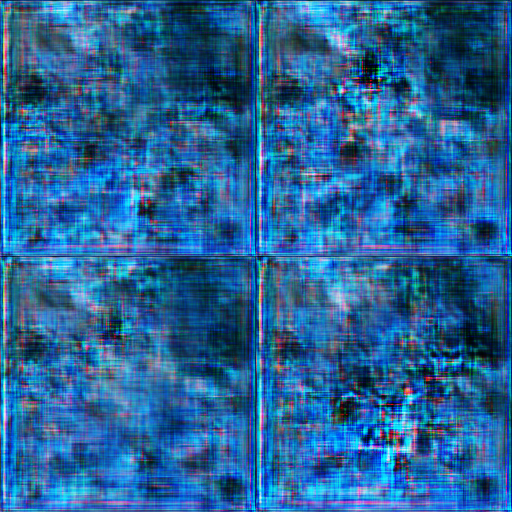
\includegraphics[clip, width=\linewidth]{fig/generative_adversarial_nets/0969_0000}
		\subcaption{epochs = 969}
		\label{fig:}
	\end{minipage}
	\begin{minipage}{0.24\columnwidth}
		\centering
		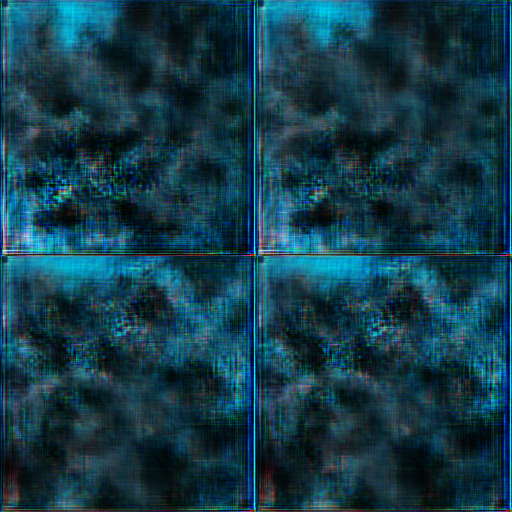
\includegraphics[clip, width=\linewidth]{fig/generative_adversarial_nets/1213_0000}
		\subcaption{epochs = 1213}
		\label{fig:}
	\end{minipage}
	\begin{minipage}{0.24\columnwidth}
		\centering
		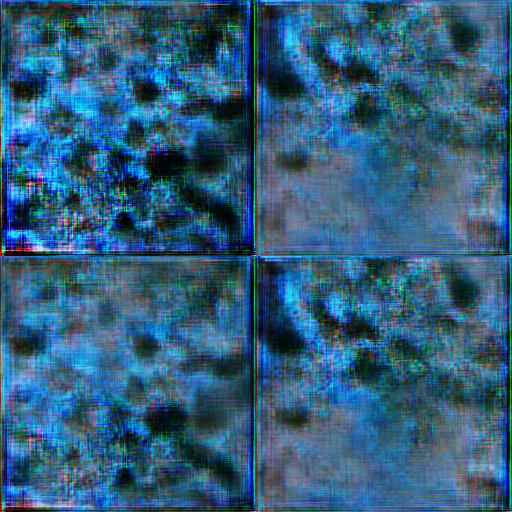
\includegraphics[clip, width=\linewidth]{fig/generative_adversarial_nets/1619_0000}
		\subcaption{epochs = 1619}
		\label{fig:}
	\end{minipage}
	\begin{minipage}{0.24\columnwidth}
		\centering
		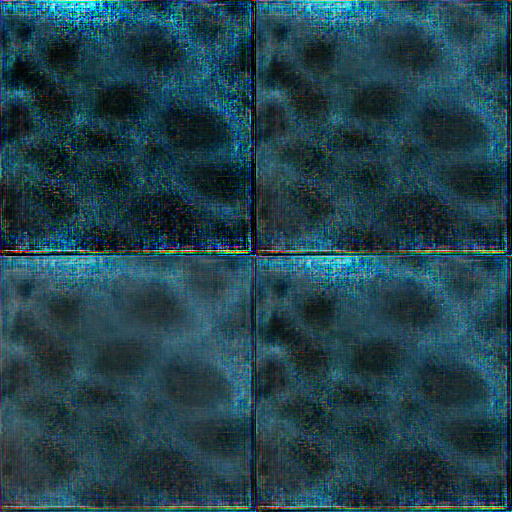
\includegraphics[clip, width=\linewidth]{fig/generative_adversarial_nets/2004_0000}
		\subcaption{epochs = 2004}
		\label{fig:}
	\end{minipage}
	\begin{minipage}{0.24\columnwidth}
		\centering
		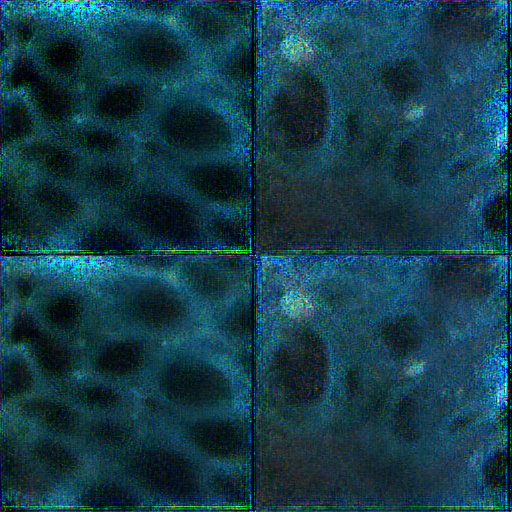
\includegraphics[clip, width=\linewidth]{fig/generative_adversarial_nets/3208_0000}
		\subcaption{epochs = 3208}
		\label{fig:}
	\end{minipage}
	
	\caption{Transition generated images by GAN}
	\label{fig:GANimage}
	
\end{figure}

\subsection{VAE}
擬似HE染色した画像と元のカラー画像のそれぞれに対してVAEを行い,潜在変数を2次元空間にプロットした結果を\fig {VAEplot}に示す.

\begin{figure}[H]
	\centering
	
	\begin{minipage}[b]{0.45\columnwidth}
		\centering
		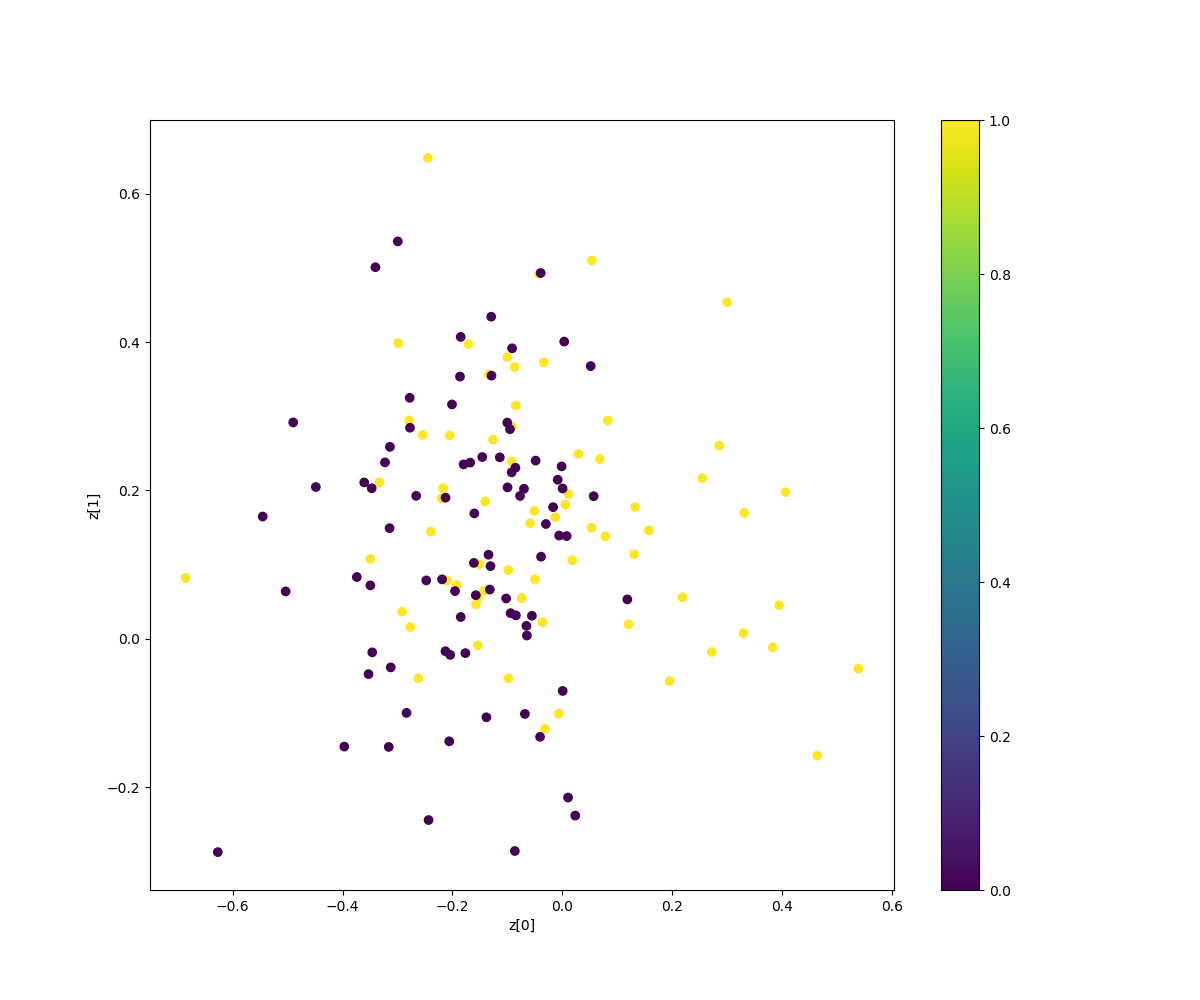
\includegraphics[clip, width=\linewidth]{fig/variational_auto_encoder/vae_colon_epoch_100_c13_he}
		\subcaption{HE like color at sample A}
		\label{fig:}
	\end{minipage}
	\begin{minipage}[b]{0.45\columnwidth}
		\centering
		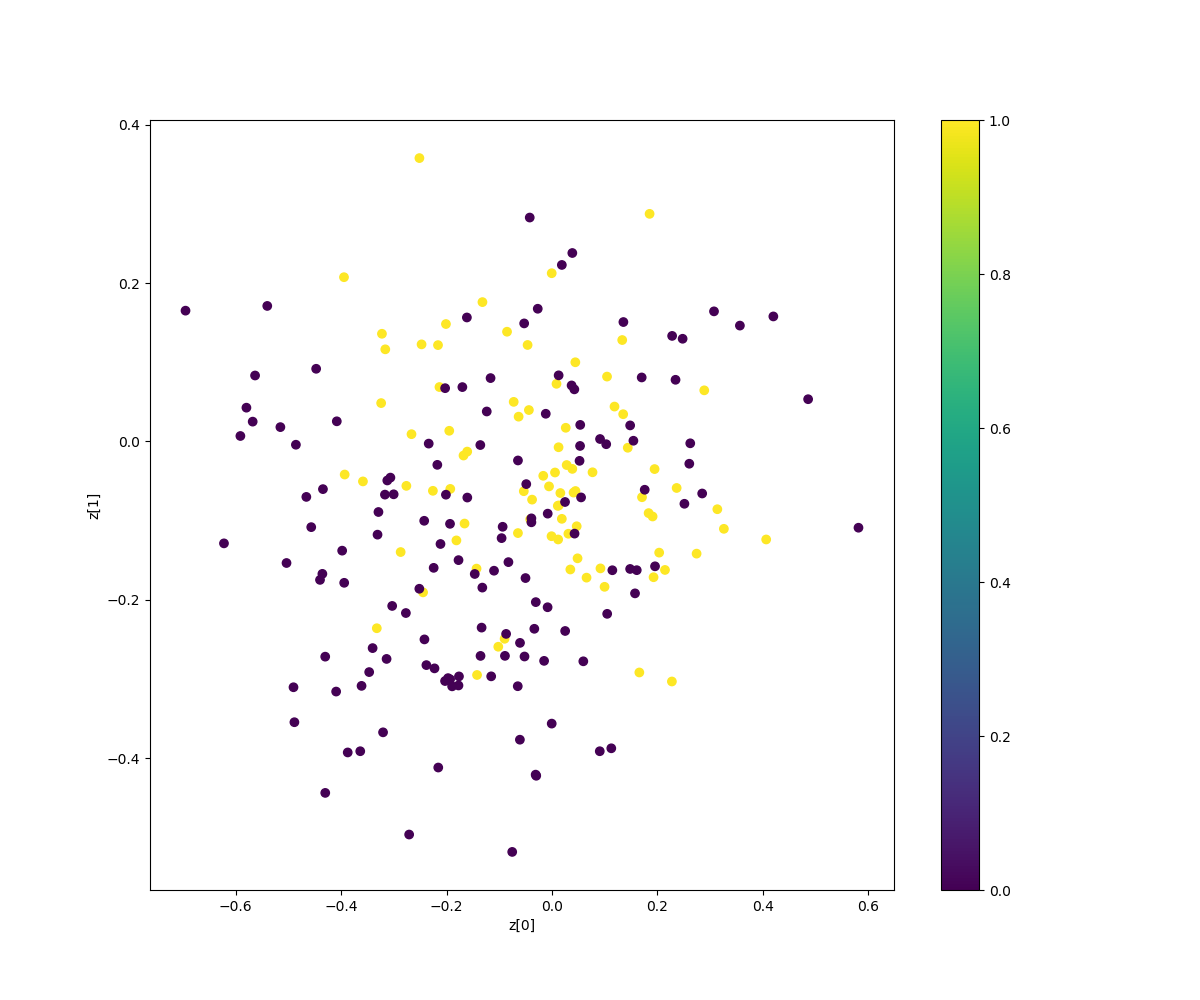
\includegraphics[clip, width=\linewidth]{fig/variational_auto_encoder/vae_colon_epoch_299_c13_rgb}
		\subcaption{original color at sample A}
		\label{fig:}
	\end{minipage}
	\begin{minipage}[b]{0.45\columnwidth}
		\centering
		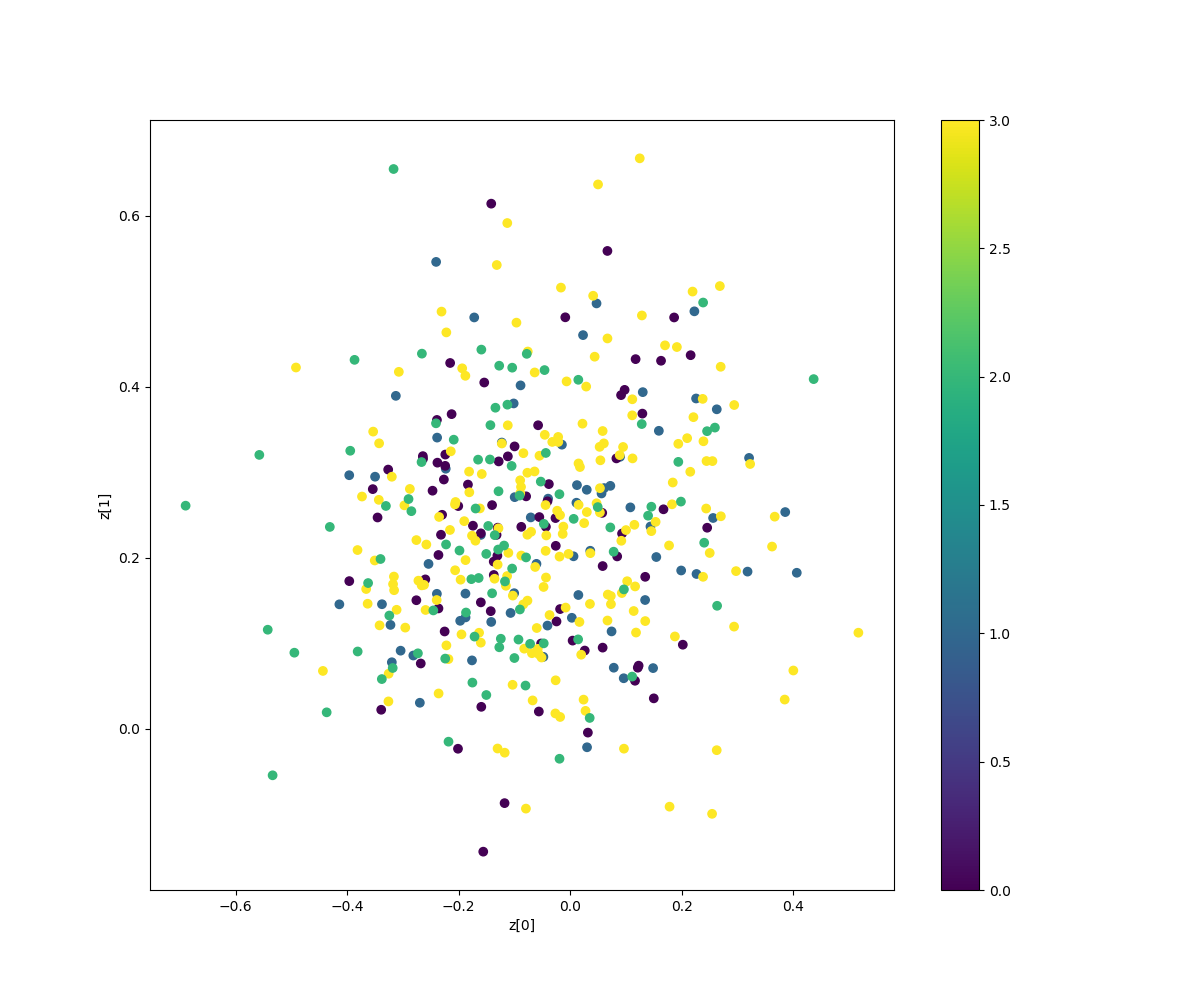
\includegraphics[clip, width=\linewidth]{fig/variational_auto_encoder/vae_colon_epoch_100_he_mix}
		\subcaption{HE like color at sample A and B}
		\label{fig:}
	\end{minipage}
	\begin{minipage}[b]{0.45\columnwidth}
		\centering
		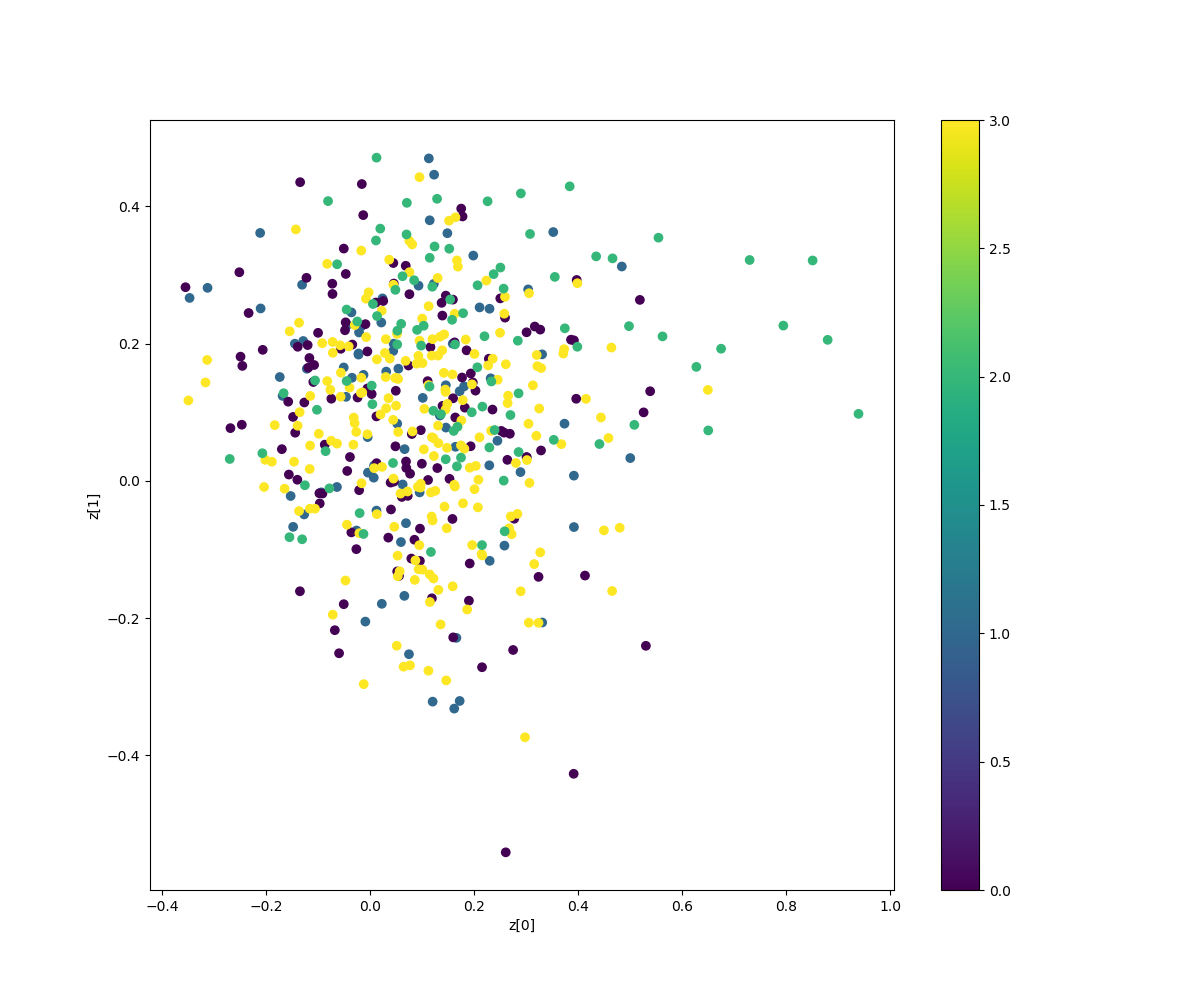
\includegraphics[clip, width=\linewidth]{fig/variational_auto_encoder/vae_colon_epoch_100_rgb_mix}
		\subcaption{original color at sample A and B}
		\label{fig:}
	\end{minipage}
	
	\caption{Latent space of 2D. Color ratio 1 is cancer, 0 is normal.}
	\label{fig:VAEplot}
	
\end{figure}

部分的には,正常と腫瘍で分布が異なるようになったが,明確な境界線を引くことが難しい.したがって,教師あり学習で境界を明確にし,教師なし学習でデータの構造を抽出することができれば,もっとも精度の高い認識モデルが作れる.

\section{半教師あり学習による識別精度評価}

\begin{figure}[H]
	\centering
	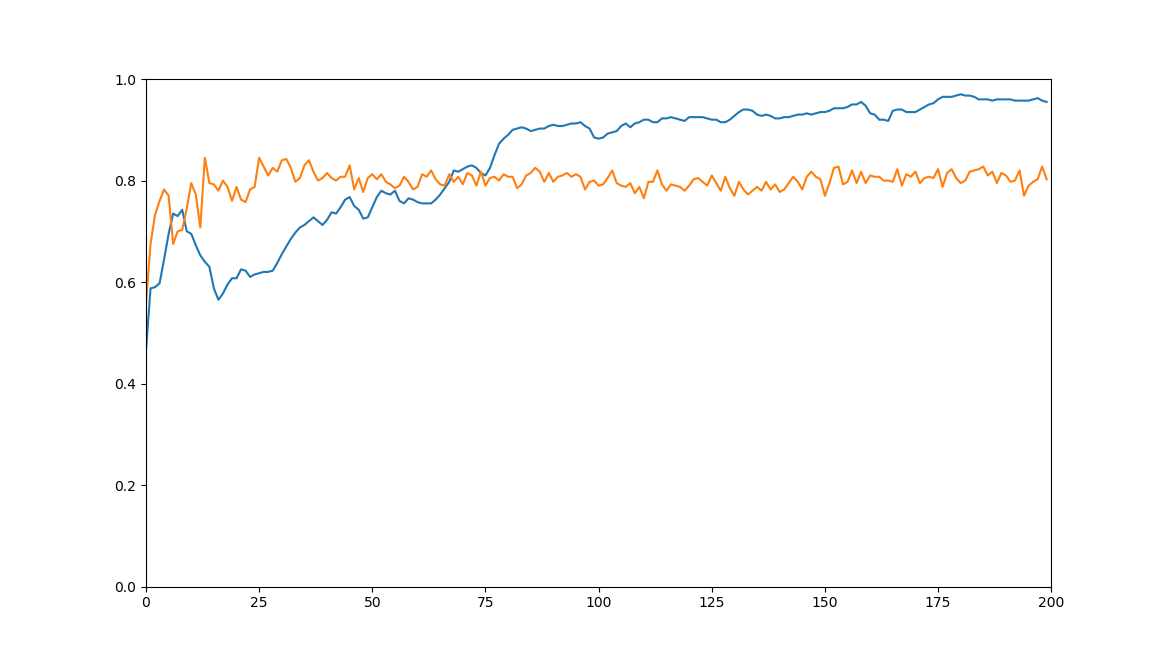
\includegraphics[width=0.7\linewidth]{fig/chapter4/accuracy_summary}
	\caption{VAE Accuracy}
	\label{fig:accuracysummary}
\end{figure}

半教師あり学習は,教師あり学習では足りない画像枚数の場合,大量の教師ラベルのない画像に対しても特徴を学習するために利用することができて,結果的に,教師ラベルの予測精度を上げることができた.


\section{学習結果の可視化}
深層学習を用いて,腫瘍らしい領域を認識するアルゴリズムを,病理医が見るために画像上に腫瘍の部分が見て分かるように可視化を行った.


まずは,スライドウィンドウで画像を取得していく.そして各ウィンドウの画像に対して病変の確率を出して,その確率をヒートマップにした.これを見て,青い領域は正常であり,黄色や赤色になっている部分が腫瘍と深層学習により認識されている部分であるため,その領域を医師が見ることでスクリーニングになり,人が見落としやすい場所に腫瘍があっても機械では見落としを防止するための診断支援に繋がる可視化にすることができた.

\begin{figure}[H]
	\centering
	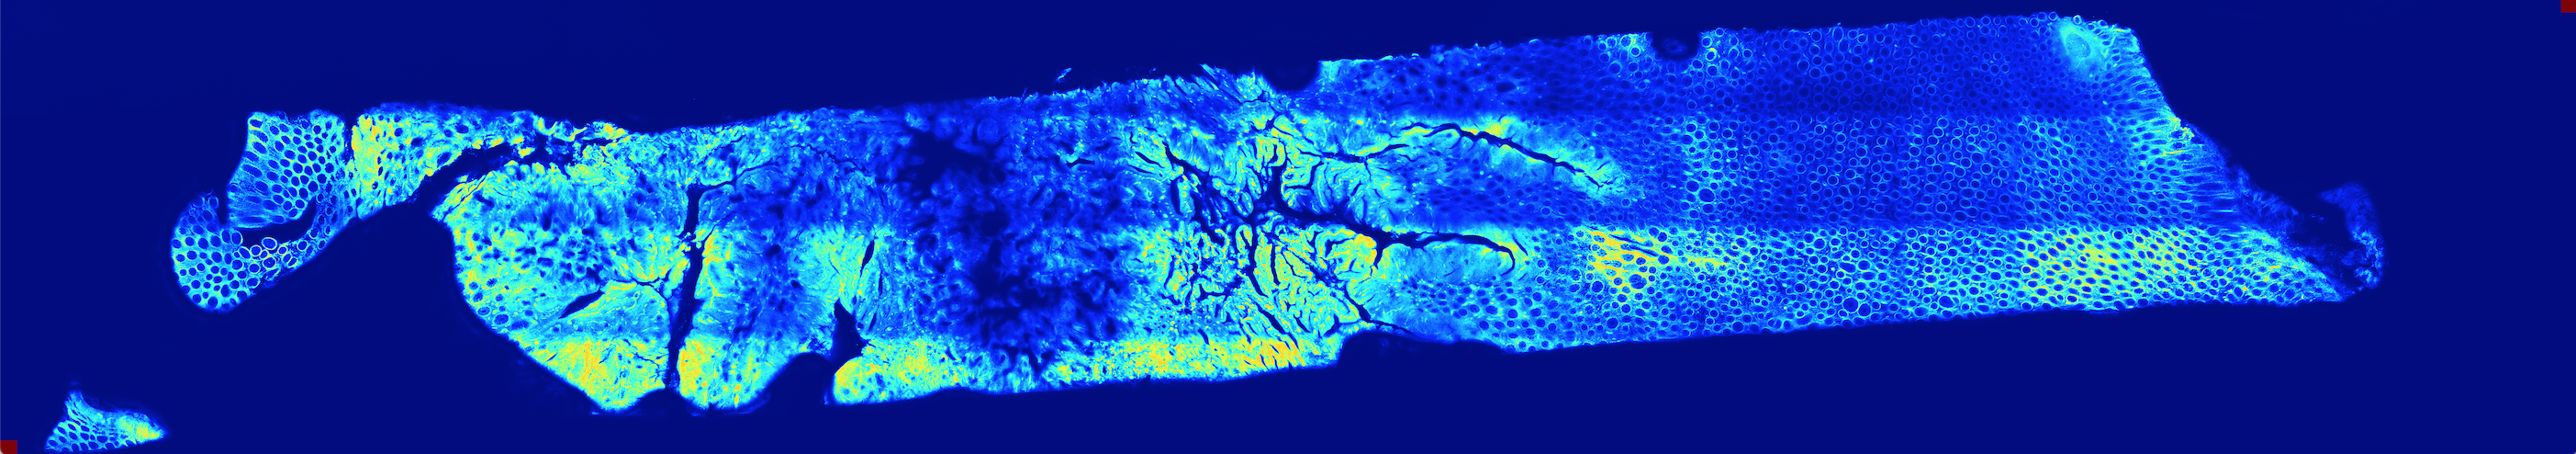
\includegraphics[width=0.7\linewidth]{fig/chapter4/visualization/sample_B}
	\caption{Visualize cancer detection}
	\label{fig:sampleb}
\end{figure}

さらにGrad-CAMを利用することでより詳細に深層学習の判断が可視化されるようになった.
\begin{figure}[H]
	\centering
	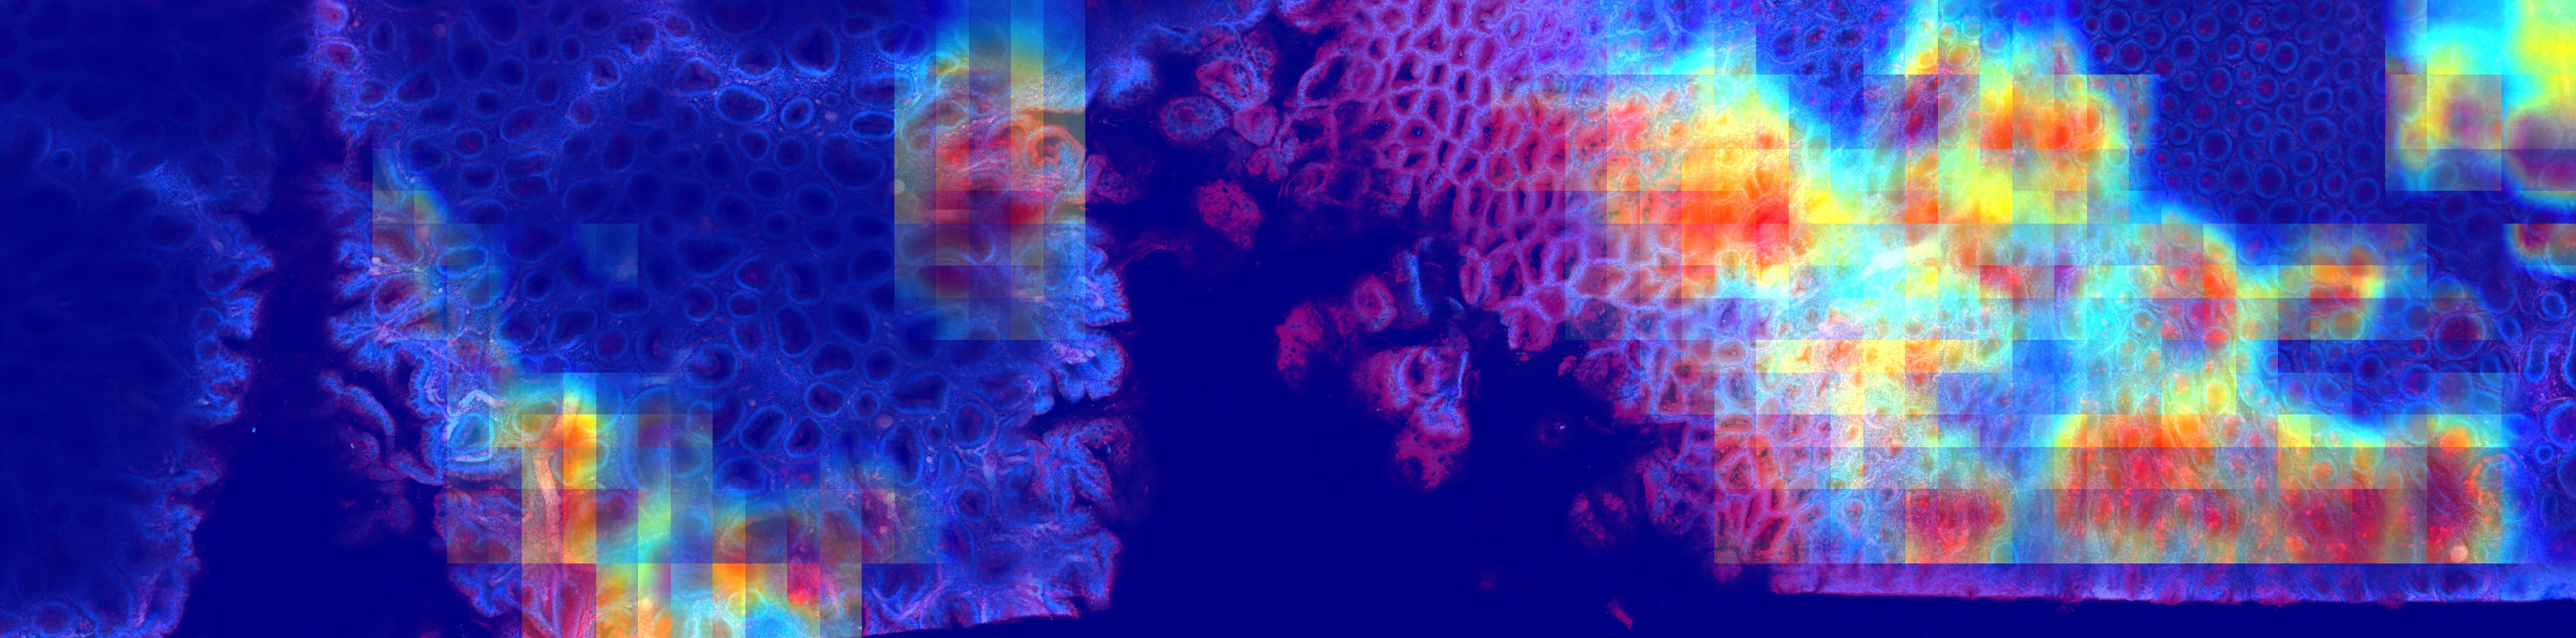
\includegraphics[width=0.7\linewidth]{fig/chapter4/large-grad-cam-step100-rm-black}
	\caption{Visualization with Grad-CAM}
	\label{fig:large-grad}
\end{figure}

\fig{large-grad}で赤色〜青色のヒートマップで塗られている部分が腫瘍であると認識された部分である.また何も塗られていない部分が正常と認識された部分である.このように可視化を行うことで腫瘍の可能性がある領域を一目で確認することができるようになった.